\section{ACAS-Xu Dataset}
\label{sect:acasxu}

ACAS stands for Airborne Collision Avoidance System. There are multiple types of ACAS benchmarks, but the one this paper is based on is Xu, which is optimized for unmanned aircraft systems (UAS), issuing turn rate advisories to remote pilots\cite{katz2017reluplex}. The installation process for the benchmark was easy, only needing to download it from GitHub\footnotemark[1].

% The files are divided into 3 components as followed:
% \subsubsection{Onnx}
% These files contain the neural network models encoded in the Open Neural Network Exchange (ONNX) format\cite{onnx}. They collectively are the core architecture for the "brain" of the benchmark, which dictates the verification and evaluation steps.
% \subsubsection{Vnnlib}
% These files contain specifications and properties that need to be verified or analyzed for the neural network models (ONNX). They contain a similar syntax to that of z3 smt-solvers.
% \newpage
% \subsubsection{Instances.csv}
% This CSV file bundles the onnx and vnnlib files into groups, where vnnlib files are associated with onnx ones. There are 10 vnnlib files and 45 onnx files, and they are combined to form a total of 186 combinations. Each combination also has metadata containing how long can the selected tool run one specific combination. 
% \\
The input data that can be found across the VNN-LIB files, revolves around different aircraft parameters determined from sensor measurements\cite{kochenderfer2011robust}. These parameters can be seen in figure \ref{fig:acasxu-geometry}:
\begin{itemize}
  \item \(\rho\) - Distance from ownership to intruder;
  \item \(\theta\) - Angle to intruder relative to aircraft heading direction length;
  \item \(\psi\) - Heading angle of intruder relative to aircraft heading direction;
  \item \(v_{\text{own}}\) - Speed of aircraft;
  \item \(v_{\text{int}}\) - Speed of intruder;
  \item \(\tau\) - Time until loss of vertical separation;
  \item \(a_{\text{prev}}\) - Previous advisory;
\end{itemize}

These values were introduced into the neural network ( the ONNX files ), representing a combination of 45 deep neural networks. The choice of having 45 DNNs comes from the need to reduce the lookup time, as previously there was only one DNN with 2GB in size \cite{katz2017reluplex}. They were created by mixing the time until loss of vertical separation (\(\tau\)) and the previous advisory (\(a_{\text{prev}}\)). Therefor every network has five inputs and five outputs. The inputs are the aforementioned ones (excluding \(\tau\) and \(a_{\text{prev}}\)), while the outputs represent the different horizontal advisories provided to the aircraft: Clear-of-Conflict (COC), weak right, strong right, weak left, or strong left. The DNNs are fully connected, use ReLU activation functions, and have six hidden layers with a total of 300 ReLU nodes each. \cite{katz2017reluplex}.

In order to confirm the correctness of the results, figure \ref{fig:acasxu-advisories} illustrates a top-down of a head-on encounter scenario, where each pixel shows a different course of action based on the presence of an intruder.

\begin{figure}[ht]
    \centering
    \begin{minipage}[b]{0.45\linewidth}
        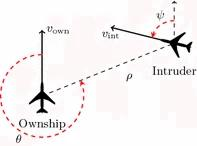
\includegraphics[width=\linewidth]{Figures/acasxu_geometry.jpg}
        \caption{Geometry of ACAS Xu horizontal logic table \cite{katz2017reluplex}}
        \label{fig:acasxu-geometry}
    \end{minipage}
    \hfill
    \begin{minipage}[b]{0.45\linewidth}
        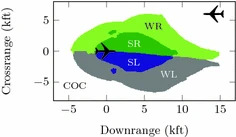
\includegraphics[width=\linewidth]{Figures/acasxu_advisories.jpg}
        \caption{Advisories for a head-on encounter with \(a_{\text{prev}}\) = COC and \(\tau\) = os \cite{katz2017reluplex}}
        \label{fig:acasxu-advisories}
    \end{minipage}
\end{figure}
